%%%%%%%%%%%%%%%%%%%%%%%%%%%%%%%%%%%%%%%%%%%%%%%%%%%%%%%%%%%%%%%%%%%%%%%%%%%%%%%%
%2345678901234567890123456789012345678901234567890123456789012345678901234567890
%        1         2         3         4         5         6         7         8

\documentclass[letterpaper, 10 pt, conference]{ieeeconf}  % Comment this line out if you need a4paper

%\documentclass[a4paper, 10pt, conference]{ieeeconf}      % Use this line for a4 paper

\IEEEoverridecommandlockouts                              % This command is only needed if 
                                                          % you want to use the \thanks command

\overrideIEEEmargins                                      % Needed to meet printer requirements.

%In case you encounter the following error:
%Error 1010 The PDF file may be corrupt (unable to open PDF file) OR
%Error 1000 An error occurred while parsing a contents stream. Unable to analyze the PDF file.
%This is a known problem with pdfLaTeX conversion filter. The file cannot be opened with acrobat reader
%Please use one of the alternatives below to circumvent this error by uncommenting one or the other
%\pdfobjcompresslevel=0
%\pdfminorversion=4

% See the \addtolength command later in the file to balance the column lengths
% on the last page of the document

\usepackage[T1]{fontenc}
\usepackage[latin9]{luainputenc}
%\usepackage[letterpaper]{geometry}
% ORIGINAL MARGINS \geometry{verbose,tmargin=2cm,bmargin=3.5cm,lmargin=2.5cm,rmargin=2.5cm}
%\geometry{verbose,tmargin=2cm,bmargin=3.5cm,lmargin=2.5cm,rmargin=2.5cm}

\usepackage{amsmath}
\usepackage{amssymb}
\usepackage{graphicx}

\makeatletter
%%%%%%%%%%%%%%%%%%%%%%%%%%%%%% User specified LaTeX commands.
\usepackage{lmodern}

\usepackage[T1]{fontenc}
\usepackage{hyperref}
\usepackage{courier}
\usepackage{color}
\usepackage{upquote}
\usepackage{xcolor}
\usepackage{listings}
\usepackage{caption}

% \hypersetup{
%     colorlinks=true,
%     linkcolor=blue,
%     filecolor=magenta,      
%     urlcolor=cyan,
% }
\usepackage[font=small,labelfont=bf]{caption}
\usepackage{bm}
\usepackage{mathtools}
\usepackage{subcaption}
\usepackage{graphicx, epstopdf}
\usepackage[framed, numbered]{matlab-prettifier}
\usepackage{flushend}
\usepackage{dsfont}
\usepackage{paralist}
\usepackage[nolist]{acronym}


% \definecolor{hellgelb}{rgb}{1,1,0.85} 
% \definecolor{colKeys}{rgb}{0,0,1} 
% \definecolor{colIdentifier}{rgb}{0,0,0} 
% \definecolor{colComments}{rgb}{0,0.5,0} 
% \definecolor{colString}{rgb}{0.81,0.12,0.95}
%  \lstset{%     
%  language=Matlab,%    
%   float=hbp,%     
%  basicstyle=\footnotesize\ttfamily,%    
%   identifierstyle=\color{colIdentifier},%    
%   keywordstyle=\color{colKeys},%    
%   stringstyle=\color{colString},%     
%  commentstyle=\itshape\color{colComments},%     
%  columns=fixed,      tabsize=4,%    
%   frame=single,%     
%  framerule=1pt,    
%   extendedchars=true,%  
%     showspaces=false,%     
%  showstringspaces=false,%      
% numbers=left,%      
% numberstyle=\tiny\ttfamily,%    
%   numbersep=1em,%    
%   breaklines=true,%  
%     breakindent=10pt,% 
%      backgroundcolor=\color{hellgelb},%  
%     breakautoindent=true,%   
%   captionpos=t,%   
%   xleftmargin=1em,%   
%   xrightmargin=\fboxsep%
% }


\newcommand{\R}{\mathbb{R}}
\newcommand{\N}{\mathbb{N}}
\newcommand{\E}{\mathbb{E}}
\newcommand{\st}{\mathrm{s.t.}}
\newcommand{\tr}{^\top}
\newcommand{\eg}{e.g.,\ }
\newcommand{\ie}{i.e.,\ }
\newcommand{\inv}{^{-1}}
\newcommand{\defeq}{\vcentcolon=}
% \newcommand\defeq{\stackrel{\mathclap{\normalfont\mbox{def}}}{=}}
% \newcommand{\red}[1]{{\color{red}#1}}
\DeclareMathOperator*{\argmax}{arg\,max}
\DeclareMathOperator*{\argmin}{arg\,min}


%%%%%%%%%%%%%%%%%%%%%%%%%%%%%%%%%%%%%%%%%%%%
% Custom Packages

% Custom Commands
\usepackage{xcolor}
\newcommand{\rohan}[1]{{\color{blue} Rohan: #1}}
\newcommand{\ali}[1]{{\color{magenta} Ali: #1}}
\newcommand{\pr}[1]{\textbf{#1:}}  % paragraph header
\newcommand{\ph}[1]{\pr{#1}} % paragraph header
\newcommand{\todo}[1]{{\color{red} #1 }} % Tasks to do
\newcommand{\inst}[1]{{\color{orange} Instructions (to be deleted asap): #1 }} %
\newcommand{\ali}[1]{{\color{cyan} Kyon: #1}}

%%%%%%%%%%%%%%%%%%%%%%%%%%%%%%%%%%%%%%%%%%%%


\title{\LARGE \bf
Autonomous Traverse of Off-road Extreme Terrains in Dark and Dust:
An Experimental Perspective on Physical Mobile Robots
}


\author{%to be ordered correctly later: David, Rohan, Jesus, Scott, Nikhi, Mike paton, Ali% <-this % stops a space
%
\thanks{$^{1}$Jesus Tordesillas is with the Aerospace Controls Laboratory, Massachusetts Institute of Technology \tt\{jtorde\}@mit.edu
       }%
\thanks{$^{2}$XX and Ali-Akbar Agha-Mohammadi are with the Jet Propulsion Lab, Pasadena, CA
        \tt\{aliagha, XXXXX\}@jpl.nasa.gov}%
}

\begin{document}

\maketitle
\thispagestyle{empty}
\pagestyle{empty}





%%%%%%%%%%%%%%%%%%%%%%%%%%%%%%%%%%%%%%%%%%%%%%%%%%
\begin{abstract}
This paper aims at pushing the boundaries of the state-of-practice in experimental autonomous traversability of extreme terrains over large, multi Km-level, scales. Specifically, we target off-road mobility-stressing terrains that include mud, rubble, high-slopes, and highly uneven surfaces. Environments are perceptually-degraded, with no GPS, variable lighting from dark to lit, and contain of obscurants (dust, fog, smoke). An important constraint for robots is to go through passages as narrow as 80cm in diameter, which limits the size of the robot and hence its sensing/computational payload power. We will focus on exploration of subsurface environments to accomplish real-world complex  missions on Earth and planetary exploration scenarios. In  particular,  we  will  discuss  the  behaviors  and  capabilities
emerge   from   the   integration   of   various layers of the  autonomy  framework ranging from mission planning, to perception, to low-level control and traversability. We  will  discuss  the  design,
hardware,  software  challenges  and traversability solutions, as well as lessons learned and future directions. We demonstrate the performance
of   the   proposed   system   and   solutions   on   physical   systems
in  real-world  relevant scenarios.
\end{abstract}

%%%%%%%%%%%%%%%%%%%%%%%%%%%%%%%%%%%%%%%%%%%%%%%%%%%%%%%%%%%%%%%%%%%%%%%%%%%%%%%%
\inst{\section{Instructions}}
%\ph{Paragraph header} Please start \uline{every single paragraph} with a paragraph header, summarizing the intention of that paragraph. This is mainly for iterations during the paper preparation. We can remove most of them for the final report.

%%%%%%%%%%%%%%%%%%%%%%%%%%%%%%%%%%%%%%%%%%%%%%%%%%
\section{Introduction}
%%%%%%%%%%%%%%%%%%%%%%%%%%%%%%%%%%%%%%%%%%%%%%%%%%%%%%%%%%%%%%%%%%%%%%%%
\todo{Ali} \ph{Real world problem and example} Consider a robot tasked to ... in a GPS-denied ... \inst{Maybe we can at the end mention DARPA is pushing to enable these behaviors by creating and organizing the subt challenge.}

\begin{figure}[t!]
    \centering
    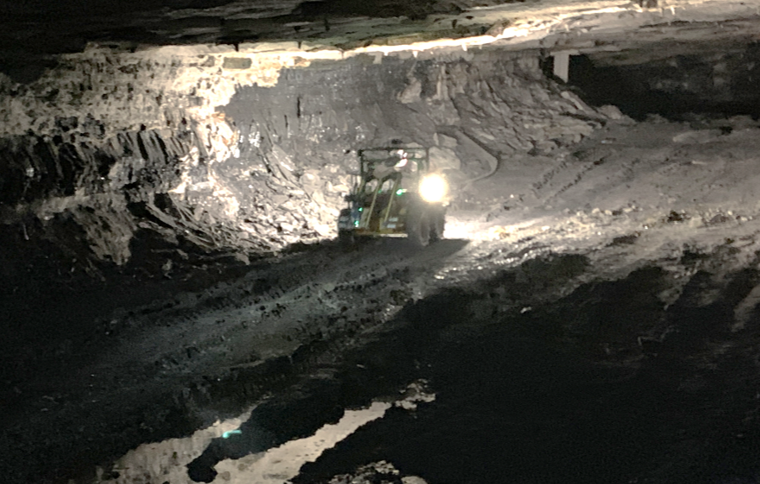
\includegraphics[width=\linewidth]{Traversability/figs/HuskyArch.png}
    \caption{Husky robot at Arch Coal Mine, West Virginia, USA.}
    \label{fig:HuskyArch}
\end{figure}

\todo{Ali} \ph{Risk-aware planning} The above problem is an instance of more generic problem of risk-aware plannign and traversability analysis... \inst{talk aobut its importnace and its general formulation (e.g., mdp, pomdp, rhc, etc).}

\todo{Ali} \ph{Challenges and gap in state-of-practice}
when deplying in the extreme environemnts and field, too much unertainty ... current methods are not sufficient...

\todo{Ali and everyone} \ph{System overview}
In this paper, we will go over a system comprised of x, y, z elements... to address this challenge in the field...

\todo{Ali and everyone} \ph{Contributions}
We push the boundaries of the state-of-practice by giving enabling .... In particular, we ...
\begin{enumerate}
    \item More accurate risk qunatitificaiton
    \item Enabling and demonstration of wheeled robotic platform to traverse terrains wiht x amount of undulation and y amount of ...
    \item Enabling and demonstration of recovery behaviors in .... and covering x amount of ground in y amount of minutes
\end{enumerate}

\ph{Outline}
Outline of the papers: related work, design principles, approach, implementation details, experimental results, conclusion

%%%%%%%%%%%%%%%%%%%%%%%%%%%%%%%%%%%%%%%%%%%%%%%%%%
\section{Problem Formulation}
\pr{State/action/observatoin}
Let $x_k$, $u_k$, $z_k$ denote the state, action, and observation at the $k$-th time step. 

\todo{david} \pr{Dynamics and observation}
\inst{add equations with uncertainty -- please look at some notation from my previous work. or let's chat on teh phone.}

\pr{environemnt model}
\inst{define the grid or however you encode the costmap}

\pr{one-step risk/cost}
$c(b,u)$ or $c(x,u)$

\pr{define path traversability index}
cost-to-go

\pr{define the traversability problem}
optimization of the index over paths

%%%%%%%%%%%%%%%%%%%%%%%%%%%%%%%%%%%%%%%%%%%%%%%%%%
\section{Architecture Overview}
% See \href{https://docs.google.com/spreadsheets/d/11qLnf_ezRuH9mCL2kmDWL4Jrx0DhV9FeSnF24StyZUg/edit#gid=0}{Literature Review}.
% See \href{https://docs.google.com/presentation/d/1zdZJyG_-8uM9AR_wMzYOIBy0c8Eg1oV7gbKtXalEBA4/edit#slide=id.g5bf125e9db_6_5}{Traversability slides}
Figure \ref{fig:ArchitectureOverview} shows an overview of the overall architecture.
Using images from camera and pointclouds from sensors the state estimator generates an estimate of the pose of the robot in $SE(3)$.
The temporal mapper fuses multiple pointclouds using these pose estimates to produce a 3D Occupancy Grid.
Next, the traversability estimator uses this occupancy grid and the most recent pointcloud to generate a costmaps at different levels of fidelity and range.
Finally, these costmaps are used by the planning layers to generate wheel velocity commands to drive the robot to the desired goal location.

\begin{figure*}[t!]
    \centering
    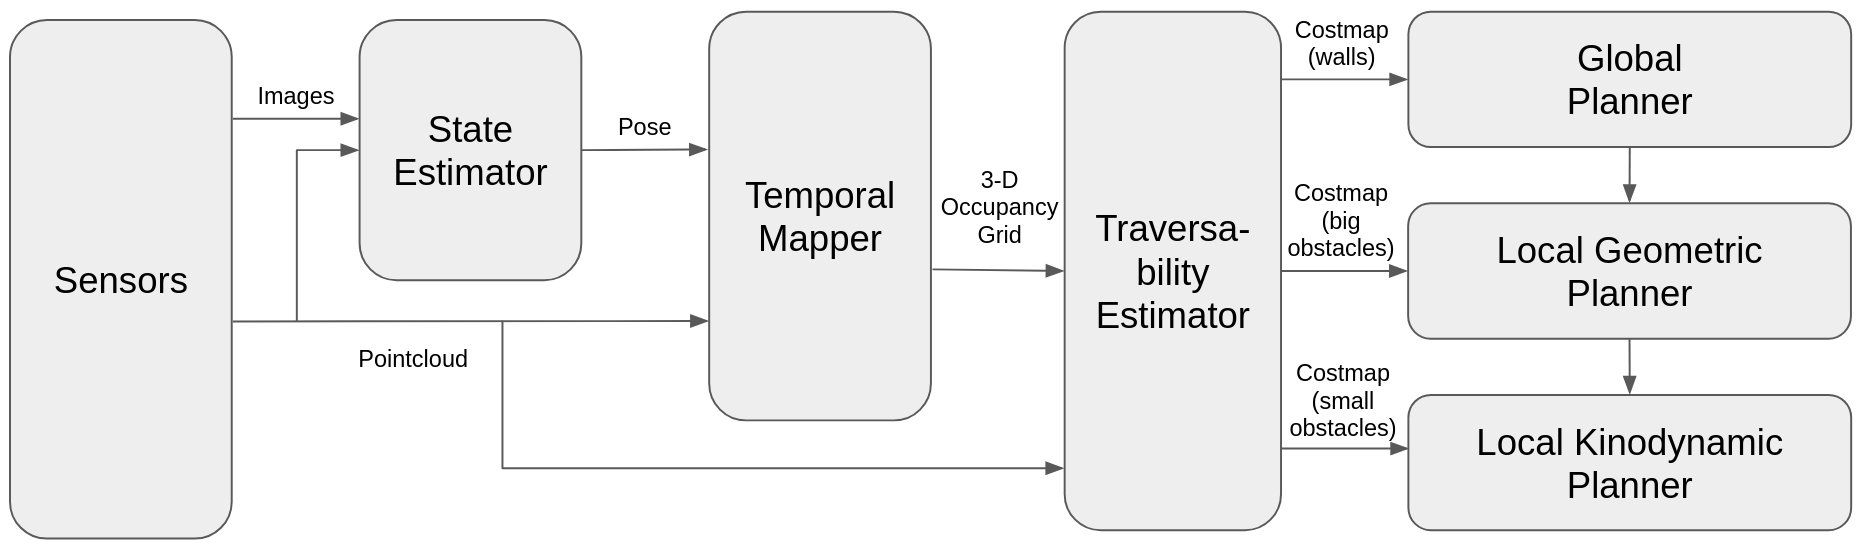
\includegraphics[width=\linewidth]{Traversability/figs/Arch.png}
    \caption{Architecture Overview}
    \label{fig:ArchitectureOverview}
\end{figure*}

%%%%%%%%%%%%%%%%%%%%%%%%%%%%%%%%%%%%%%%%%%%%%%%%%%
\section{Dealing with Uncertainty}
blah blah

\subsection{Challenges}
\begin{itemize}
    \item Darkness
    \item Dust
    \item Self-similar environments
    \item Rough Terrain
    \item High slippage (Mud, Sand)
    \item Negative Obstacles
    \item Limited Comms
    \item Unknown, unmapped environments
\end{itemize}

\pr{Whats the Challenge}
As shown in Fig.~\ref{fig:HuskyArch}, low-lighting, dust and rough terrain are key features of subterranean environments which make state estimation and mapping really challenging.
Errors in perception percolate to the planner and controller and eventually can lead to failure of the complete system. 

\pr{How do we solve it}
To address this issue we developed a robust state estimator which leverages redundancy and heterogeneity.

\subsection{Heterogeneous Redundant Odometry (HeRO)}
\pr{Failures and philosophy}
State estimation failures can be triggered by many factors like dust, low-light conditions, lack of features/landmarks, dynamic range issues in cameras, presence of symmetries in environments for lidar-based localization, etc.
HeRO \cite{hero2019isrr} is a state estimator designed to achieves robustness to these failures by exploiting redundancy and heterogeneity in sensing and odometry algorithms. 

\pr{Algorithm details}
The robot is equipped with redundant cameras and lidars of different wavelengths pointing in different directions to maximize the field-of-view.
Many camera's such as Intel Realsense T265 or Qualcomm snapdragon flight are equipped with on-board state estimators. 
HeRO is designed to leverage these robust commercial implementations of state estimators and multiplexes a continuous pose estimate from the most reliable source from these redundant estimates by performing confidence tests.

\subsection{Multi-fidelity Traversability Estimator}

\pr{Why multi-fidelity?} 
While HeRO provides robustness to complete loss of state estimates in several failure modes, the estimates still lack accuracy due to presence of drift in pose estimates.
This drift in estimated pose ends up corrupting the temporal map.
This implies that there is a trade-off between accuracy of the map and it's range.
To get larger range, more pointclouds need to be fused by using more number of noisy pose estimates leading to lesser accuracy. 
Traversability estimator produces a costmap using the occupancy grid from the temporal mapper.

\pr{Why stochastic maps are not enough}
The stochastic temporal maps that implement belief updates such as log-odds \cite{hornung2013octomap} partially mitigate this issue.
However, like any other filter, optimizing the belief update parameters to remove noise introduces a lag in the estimates.
Hence, our traversability estimator balances the trade-off between range and accuracy by producing maps at multiple fidelities as shown in Fig.~\ref{fig:costmap}. 

\begin{figure}[h!]
    \centering
    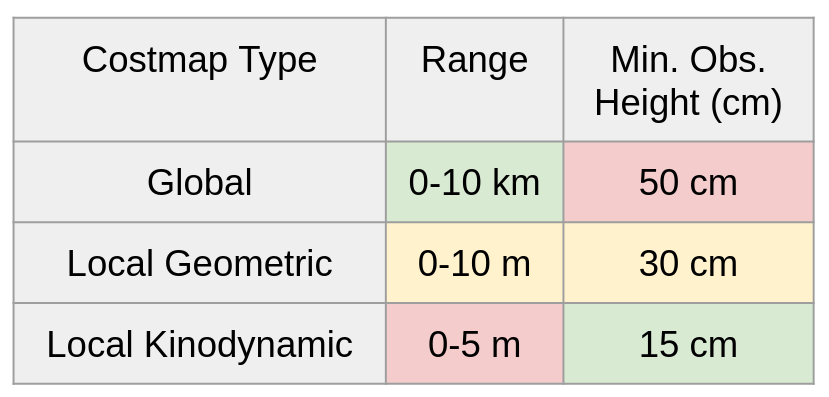
\includegraphics[width=\linewidth]{Traversability/figs/Costmap.png}
    \caption{Fidelity levels of costmap to balance range-accuracy trade-off.}
    \label{fig:costmap}
\end{figure}

\pr{Instantaneous Pointcloud Idea}
Note that the costmap for the local kinodyanmic planner, designed to detect the smallest obstacles, doesn't use the temporal map at all.
A key idea to enable this was to re-plan short-range trajectories at high-speed in body frame using the most recent pointcloud \cite{instantaneousPointclouds}.
Furthermore, we need to ensure that a single scan provides sufficiently large field-of-view to ensure the set of trajectories are not too restrictive.
Hence, the robot was equipped with three Velodyne VLP16 lidars.

For larger obstacles, relying on instantaneous pointcloud data from sensors which provide good coverage of the surrounding environment is sufficient.  However, due to the presence of blindspots or sparse lidar data, detecting small obstacles can be difficult due to insufficient data.  To address this issue, we fuse the past 1-5 seconds of lidar data which provides a richer and more complete picture of the environment.  The longer this temporal window is, the more susceptible to localization noise our costmap will be.  Therefore if our state estimator HeRO detects a failure or decrease in confidence, this temporal window can be dynamically reduced.

\pr{Negative Obstacles}
Since detecting negative obstacles is vital to preserving the life and safety of the robot, we apply the idea of relying on instantaneous (or temporally fused) pointclouds and detect negative obstacles without having to rely on accurate localization.  This eliminates the possibility that errors in localization will create virtual floors which the robot may wish to drive over.  We take a simple geometric approach which detects gaps in the pointcloud which correspond to negative obstacles.  Negative obstacles which do appear in the pointcloud are not handled with this approach, and are instead detected via the settling algorithm outlined in the next section.

\pr{Settling Algorithm}
Traversability at different query points on the costmap is obtained by running a 3-D settling algorithm \cite{krusi2017driving}.
For a given query pose in $SE(2)$, a settled pose in $SE(3)$ is computed by settling the robot on the ground to obtain its height, roll and pitch.


\subsection{Recovery Behaviors}
In the real world, failures are unavoidable. 
Hence, as a last line-of-attack, we design behaviors to recover the system from failures.
The following recovery behaviors are triggered (in described order) when the any local planner fails to find a path:
\begin{itemize}
    \item Clearing the temporal map and start building it from scratch. 
    \item Rotate the robot, open-loop, in the direction of maximum clearance.
    \item Terminate current goal and return to base.
    \item Backwards wall-follow (implemented by giving a carrot goal in body frame).
\end{itemize}


\begin{figure*}[b]

\centering
\includegraphics[width=.32\textwidth]{figs/mud1.png}\hfill
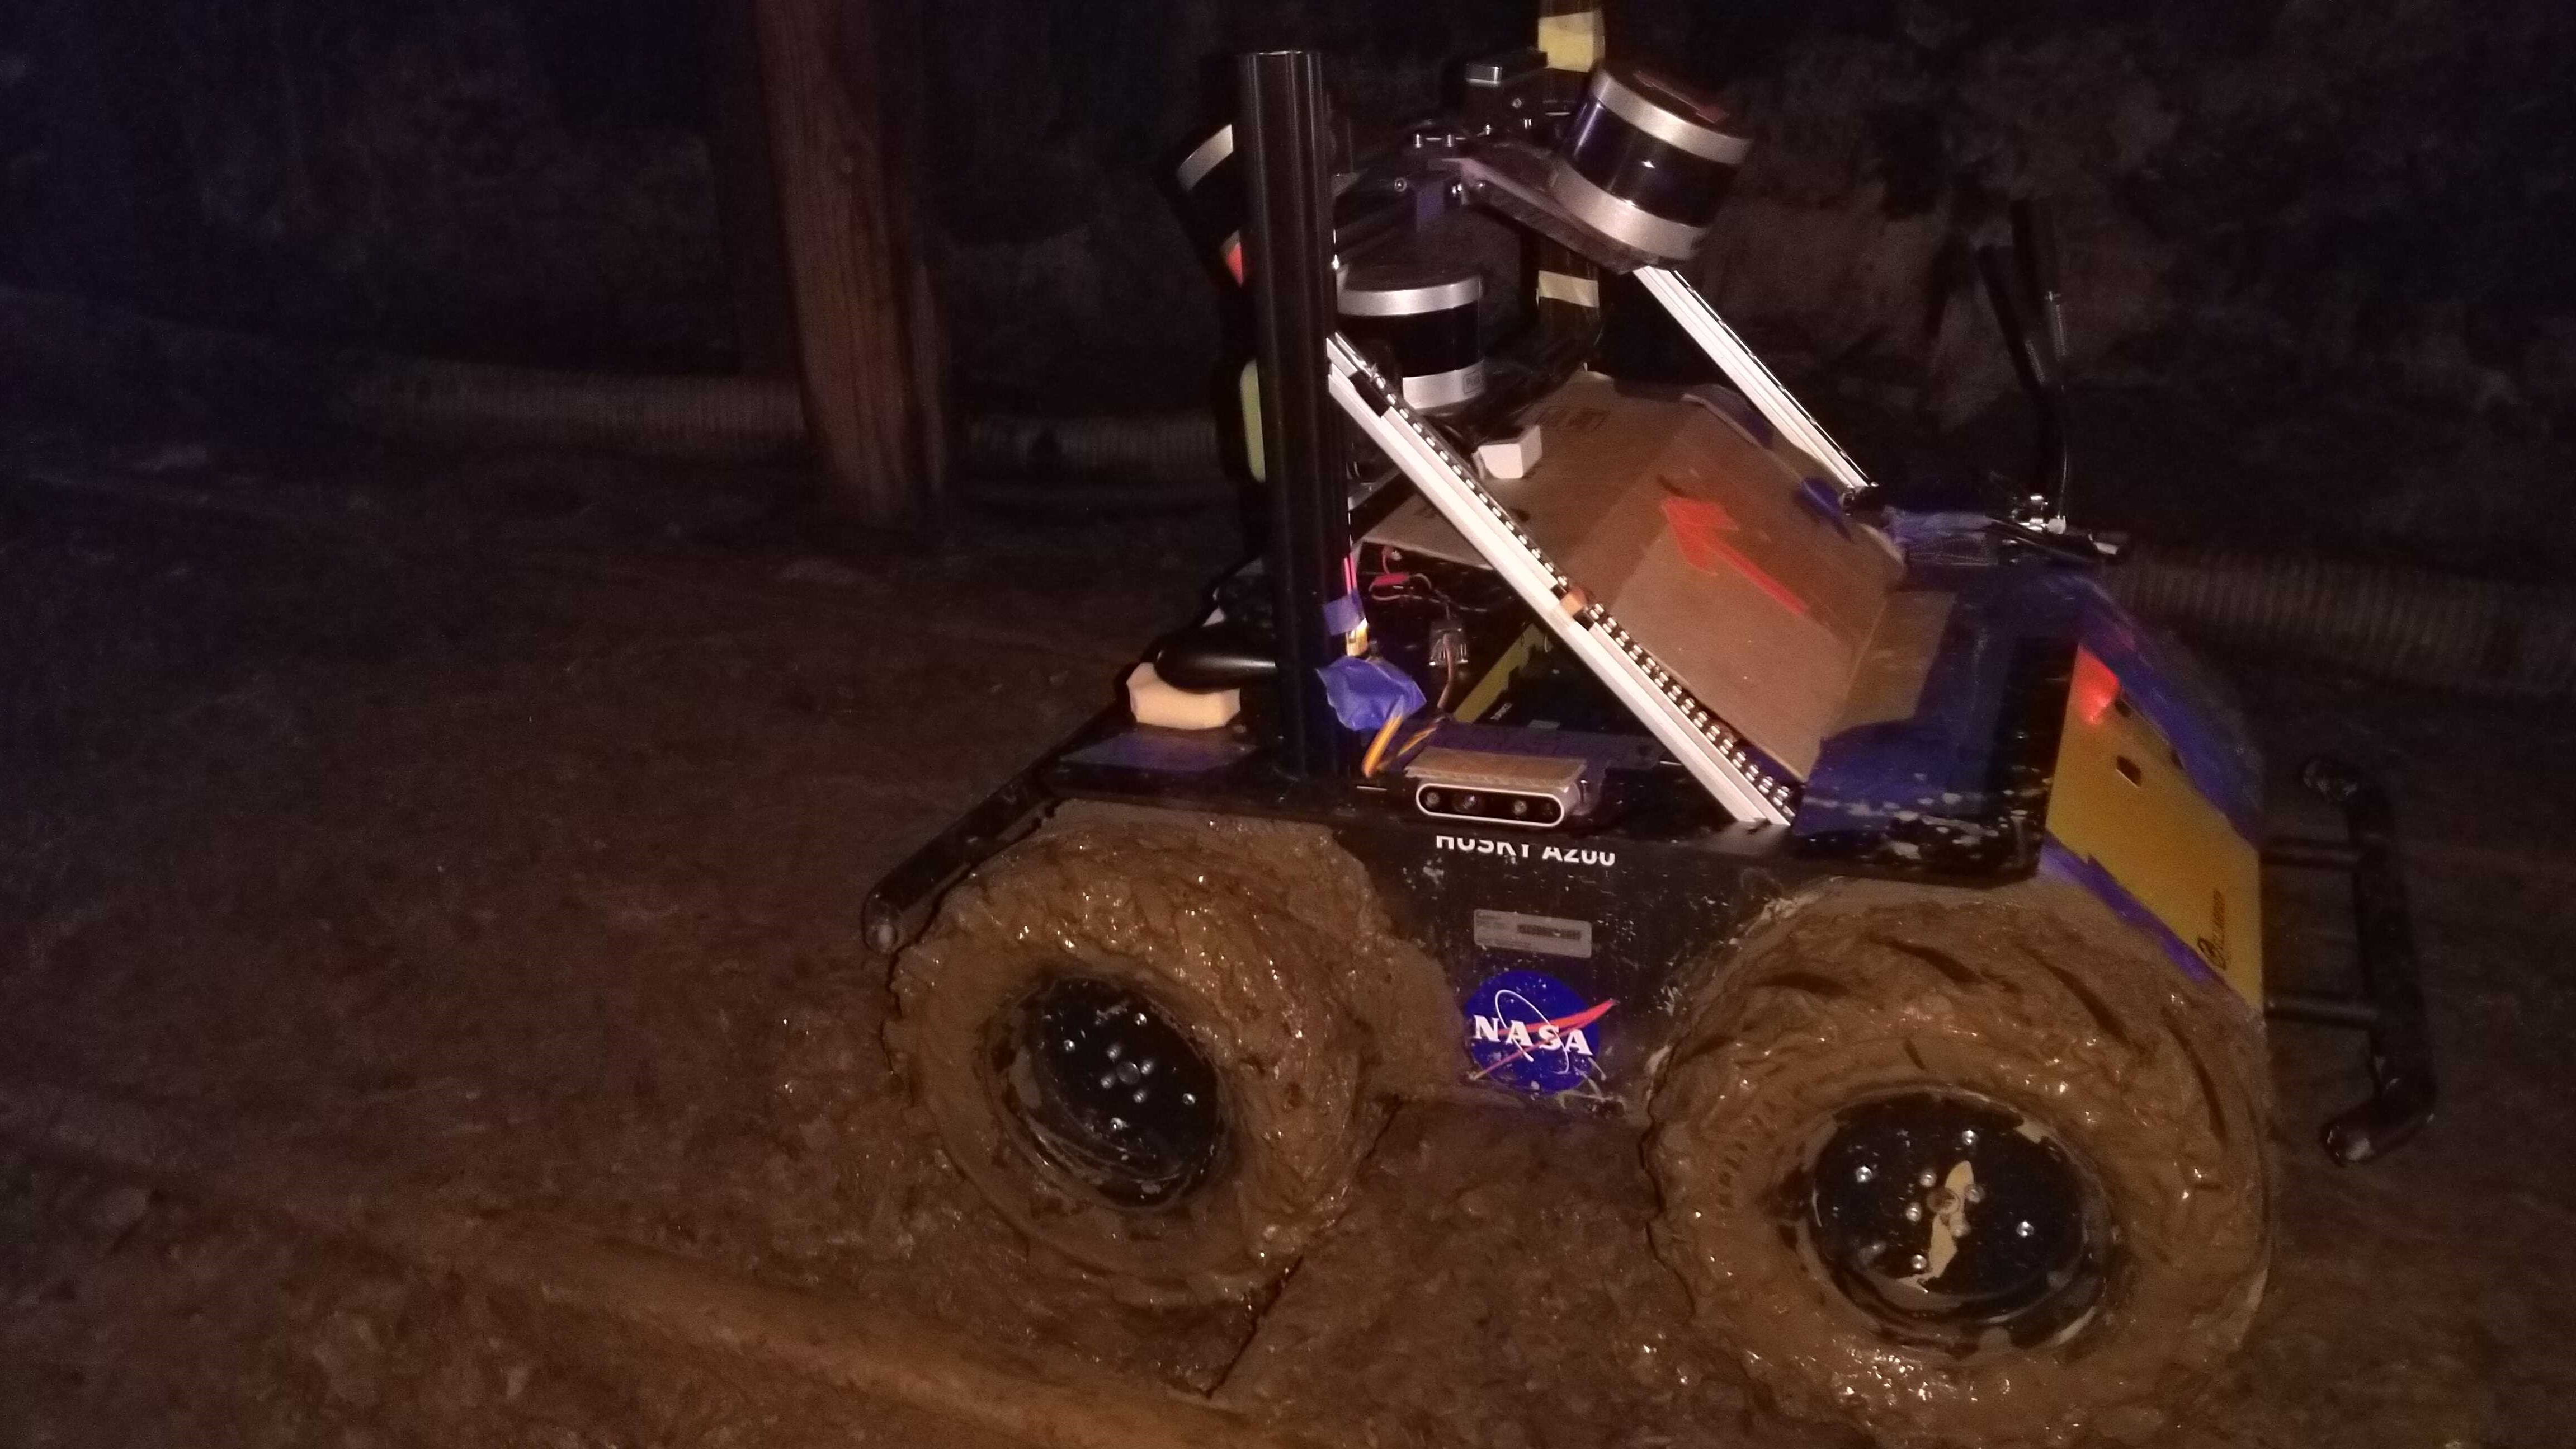
\includegraphics[width=.32\textwidth]{figs/mud2.jpg}\hfill
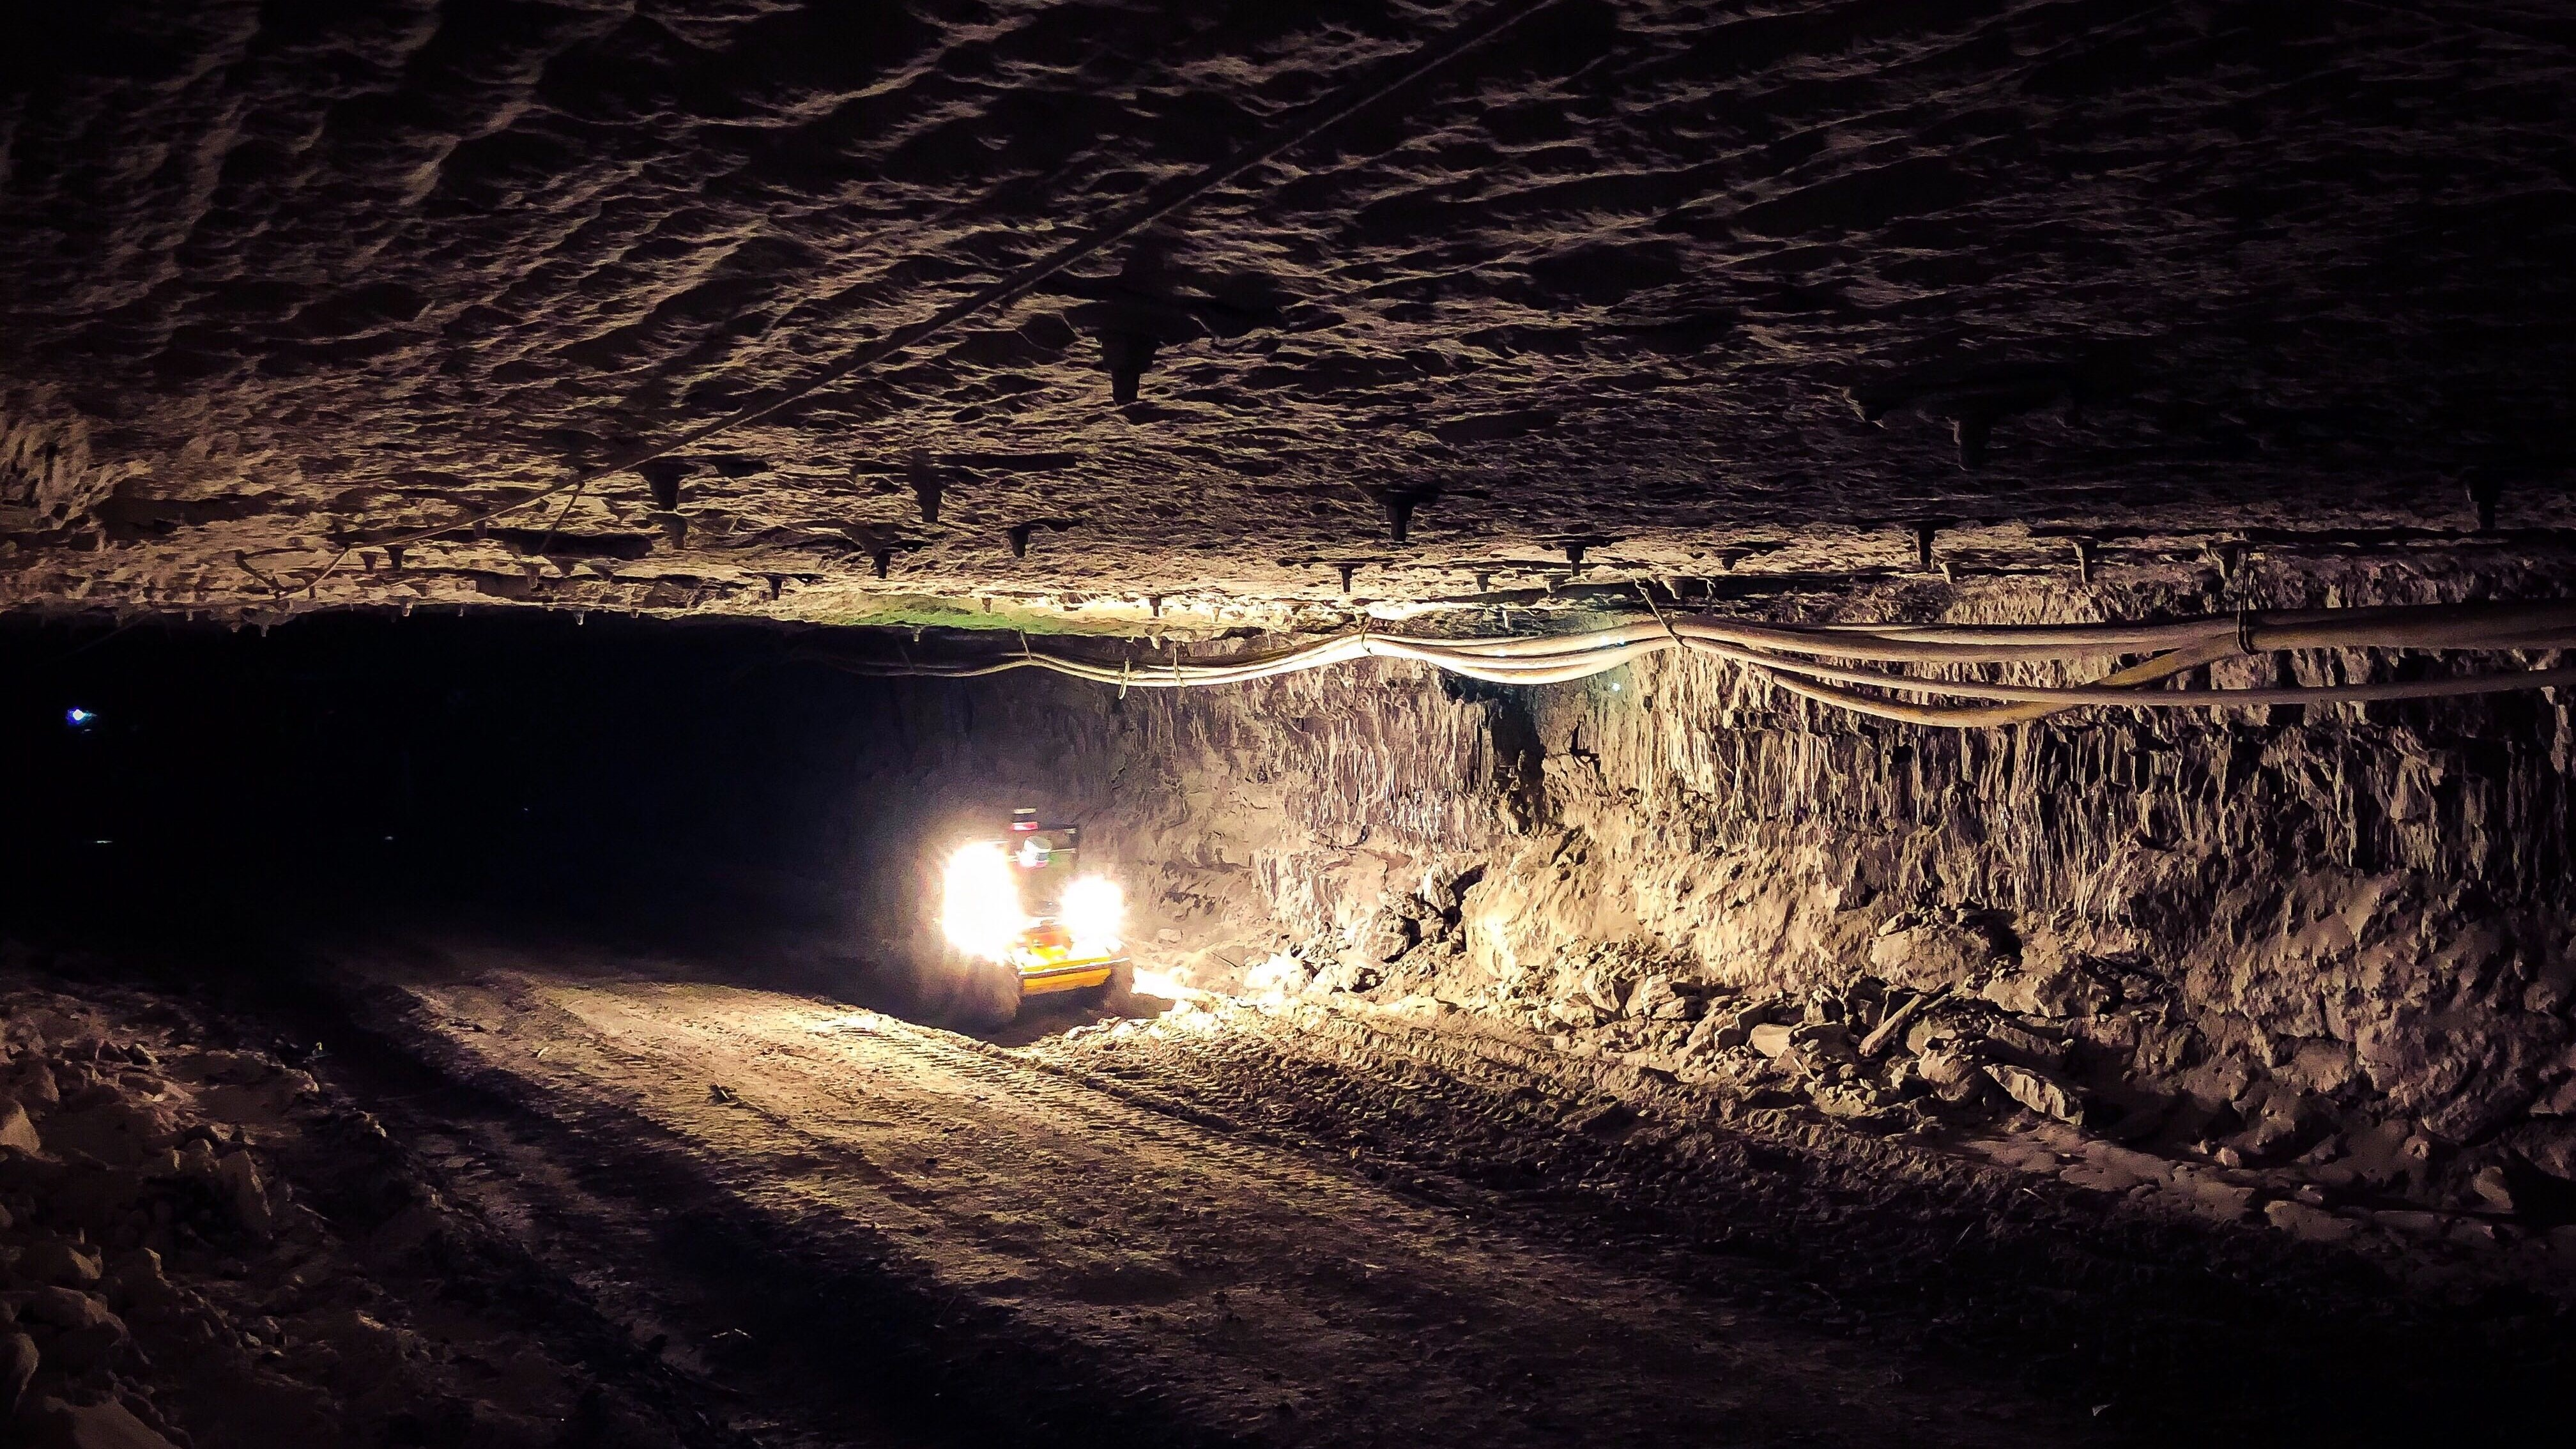
\includegraphics[width=.32\textwidth]{figs/arch1.jpg}

\caption{default}
\label{fig:figure3}

\end{figure*}


\section{Local Planning}
Assessing traversability and risk is prerequisite to autonomous navigation in extreme environments.  These traversability challenges, which have to be accounted for by a local planner, include high slopes, obstacles, holes, comm nodes dropped by the robot or sensor blind spots.  In order to find a balance between efficient traversal and low risk to the platform, we construct a measure of accumulative risk for a given path through the environment.  Let $g=(m^1,\cdots,m^n)$ be a grid of $n=n_l\times n_w$ cells with length $n_l$ and width $n_w$, and let each $m^i\in[0,1]$ represent the probability that the robot safely traverses through the cell.  Let $\pi=\{i_t\}_{t=0}^T$ be a sequence which defines a connected path through the grid, and define the solution space $\Pi$ as the set of connected paths through the grid which connects the current robot position with the goal.  Then we define the total accumulated risk of the path $\pi\in\Pi$ as 
\begin{align}
 \mathcal{R}^{\pi}=1-\prod_{t=0}^Tm^{i_t}
\end{align}
which is the probability that the robot fails to safely traverse the path $\pi$.  


%\ph{Sources of Risk}
We combine multiple layers of grids which encode different types of risk.  Assuming mutual exclusivity between each risk type, the total risk in each grid cell is simply the product of the individual risks of each layer.  We consider the following sources of risk:
\begin{itemize}
    \item Obstacles (Walls, Rubble, etc.)
    \item Steep Slopes
    \item Negative Obstacles
    \item Sensor Blind Spots
    \item Mission Items (comm nodes, other robots, etc.)
\end{itemize}
To identify these sources of risk, we perform traversability analysis on a local map generated from KO/VO odometry and sensor measurements (depth camera, LiDAR).  We fit local ground planes on the map to identify traversable ground regions.  Ground planes which have too high of a slope are identified as ``Steep Slope" regions.  Points on the map which are above or below the ground plane which are higher than the ground clearance of the robot are marked as ``Obstacles".  Negative obstacles are identified by gaps in the map (where no sensor measurements are available).  Sensor blind spots contribute a non-lethal risk and are identified by the respective sensor models.  Finally, we add mission-specific items to the risk map (to avoid dropped comm nodes, other robots, etc.) For an example of the risk mapping identifying obstacles, see Figure \ref{global_costmap}.

\begin{figure}[thpb]
   \centering
    \begin{subfigure}{0.5\linewidth}
        \centering
        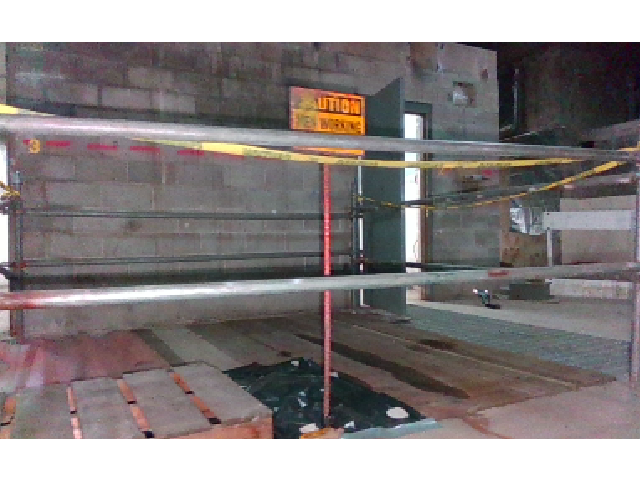
\includegraphics[trim={1cm 1cm 0cm 1cm},clip, width=\linewidth]{figs/costmap_image.png}
    \end{subfigure}%
    ~ 
    \begin{subfigure}{0.5\linewidth}
        \centering
        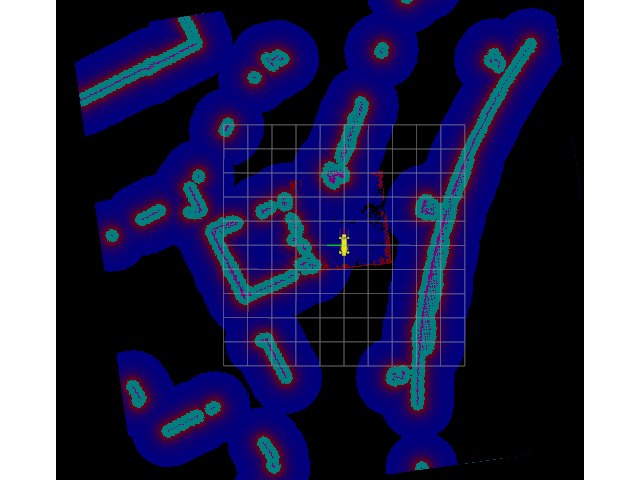
\includegraphics[trim={1cm 1cm 1cm 2cm},clip,width=\linewidth]{figs/costmap_large.png}
    \end{subfigure}
    \caption{Left: left camera image of a high-risk traversable region.  Right:  Risk map with obstacles in image to the left of the robot (centered); 1m markings are in gray.}
    \label{global_costmap}
\end{figure}


%Accurate risk assessment is contingent upon good localization/odometry.  When odometry fails we want our assessment of risk to remain conservative in such a way as to keep the vehicle safe at all times.  Therefore we rely on a multi-resolution approach for assessing risk.  We asses risk on a local scale (2m radius) by relying on wide-field of view sensor data with a short temporal window.  This approach relies on a short history of KO/VO odometry, which tends to have low drift at these timescales.  For areas outside this small radius (2m-10m), we rely on temporally fused sensor data using our LiDAR payload, since this sensor has much longer range and higher accuracy at these scales.  We combine these two layers to achieve both long-range mapping for efficient planning, along with high-fidelity mapping at short ranges to ensure the safety of the platform.

%\ph{Solver}
We search for the minimum risk path using A*:
\begin{align}
    \pi^* = \arg\min_{\pi\in\Pi}\mathcal{R}^{\pi}(g)
    \label{deterministic_plan}
\end{align}
Having found the minimum risk path, we then send a carrot waypoint 1m along this path to the low-level controller of the legged system. The low-level controller in the Spot robot received information from Spot's sensors (not the payload sensors). Due to the configuration of Spot cameras and their limited field of view, it is much safer and more effective for the robot to prefer moving in the forward direction, where sensor coverage is better.  In general, within the NeBula framework, we formalize this notion with a perception-aware planner.

%\ph{Uncertainty-aware Representation}
We model each cell $m^i$ as a random variable, where $\hat{m}^i$ and $\sigma^{m^i}$ denote its mean and variance. The ``information" about $m^i$ is captured in the $\sigma^i$, where fully unknown and fully known cells have the highest and lowest $\sigma^i$ values, respectively.  By explicitly capturing the learned information about each cell $m^i$, we can treat all the cells (known, unknown, partially-known) in a unified manner. 

%\ph{Uncertainty-aware map prediction}
This representation allows us to incorporate perceptual capabilities %(hence the name "perceptual" in NeBula) 
into the planning. Given the sensors available on the robot and their configuration and noise characteristics, we can derive models that predict the evolution of $\sigma^i$ based on the sensor configuration and most likely measurements along a given trajectory $\pi$. 
\begin{align}
 \sigma^i_k = \tau( \sigma^i_0, z_{0:k}(\pi) )
\end{align}
where the measurements $z_0,\cdots,z_k$ are predicted at each of the first $k$ time steps along the path $\pi$.
This becomes increasingly important when the sensor configuration is highly asymmetric on a robot, which is the case for Spot as it has blind spots and areas where sensory measurement noise is considerably higher than other areas.  We denote the predicted map $k$ time steps in the future along the trajectory $\pi$ by 
\begin{align}
 g_k = \{p(m|m^1_k,\sigma^1_k),\cdots,p(m|m^n_k,\sigma^n_k)\}   
\end{align}
where $p(m|m^i_k,\sigma^i_k)$ is the probability distribution of $m^i$ parameterized by $m^i_k$ and $\sigma^i_k$.
As a result, we define a risk measure that takes perceptual capabilities and uncertainties into account when planning trajectories, by minimizing accordingly:
\begin{align}
 \mathcal{R}_k^{\pi}=1-\prod_{t=0}^Tp(m|m_k^{i_t},\sigma_k^{i_t}),~~~
    \pi^* = \arg\min_{\pi\in\Pi}\mathbb{E}[\mathcal{R}_k^{\pi}(g_k)]
\end{align}
Efficient methods for computing predicted risk uncertainty over a 2-D grid for a given sensor model have been considered in \cite{CRM}.
%Ali-akbar Agha-mohammadi, Eric Heiden, Karol Hausman and Gaurav S. Sukhatme, “Confidence-rich 3D Grid Mapping: Toward High-speed Vision-based UAV Navigation,” International Journal of Robotics Research (IJRR), vol.38, pp.1352-1374, 2019.


%\ph{Specific example Necessity of perception aware planing in Spot}
%Although a key feature of NeBula is in planning perception-aware paths, 
To realized this behavior, in the case of integration of NeBula with Spot, we found that a simple heuristic sufficed to approximate the optimal solution $\pi^*$.  This heuristic was to solve for deterministic A* paths (Equation \ref{deterministic_plan}) and then to give a desired location and orientation to Spot as a waypoint along this path, such that the relative heading between the current robot position and the waypoint itself is minimized. This results in a behavior where the robot orients itself forward as it walks whenever possible. Holonomicity of the robot allows us it to orient itself in any direction as it moves.  Furthermore, the sensor coverage from Spot's internal cameras is good in the near-field, while the onboard LiDAR on the NeBula payload is good in the far field.  We combine these two streams of data to compute risk (see Figure \ref{bd_costmap}).  Future work will involve bringing the more advanced uncertainty-aware planning from the NeBula framework into Spot. 

\begin{figure}[thpb]
   \centering
    \begin{subfigure}{0.5\linewidth}
        \centering
        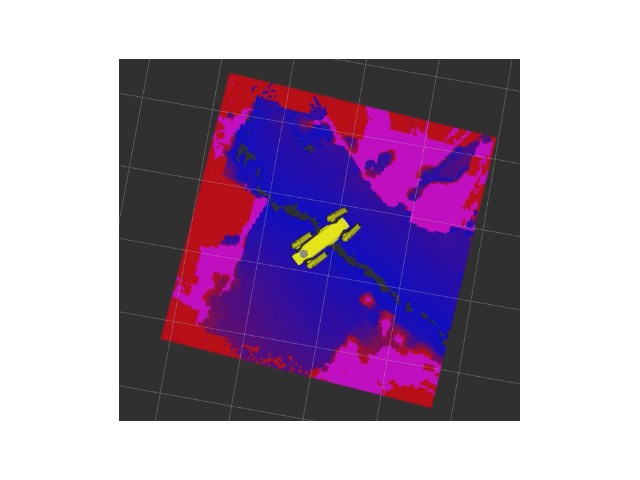
\includegraphics[trim={4cm 3cm 4cm 3.5cm},clip, width=\linewidth]{figs/costmap_bd2.png}
    \end{subfigure}%
    ~
    \begin{subfigure}{0.5\linewidth}
        \centering
        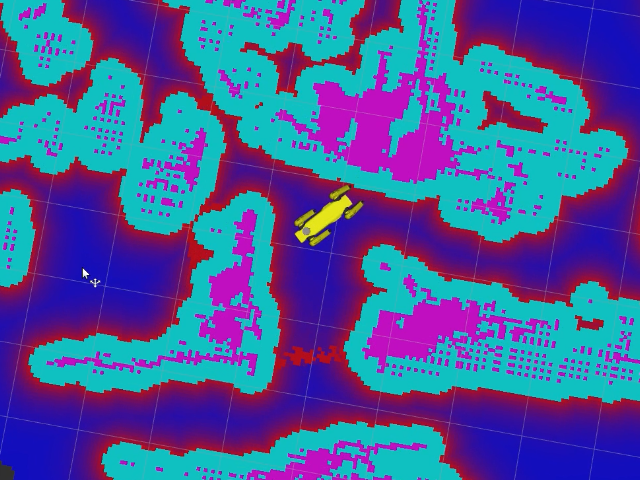
\includegraphics[trim={1cm 1cm 1cm 1cm},clip, width=\linewidth]{figs/costmap_bd2_embedded.png}
    \end{subfigure}
    \caption{Left:  Risk map generated from Spot's onboard cameras with lethal (pink), high-risk but non lethal (red), and low risk (blue) regions. Right: Spot risk map layer combined with LiDAR based risk map showing larger range of obstacles for a more robust and long-range planning.}
    \label{bd_costmap}
\end{figure}

\begin{figure}[thpb]
    \centering
    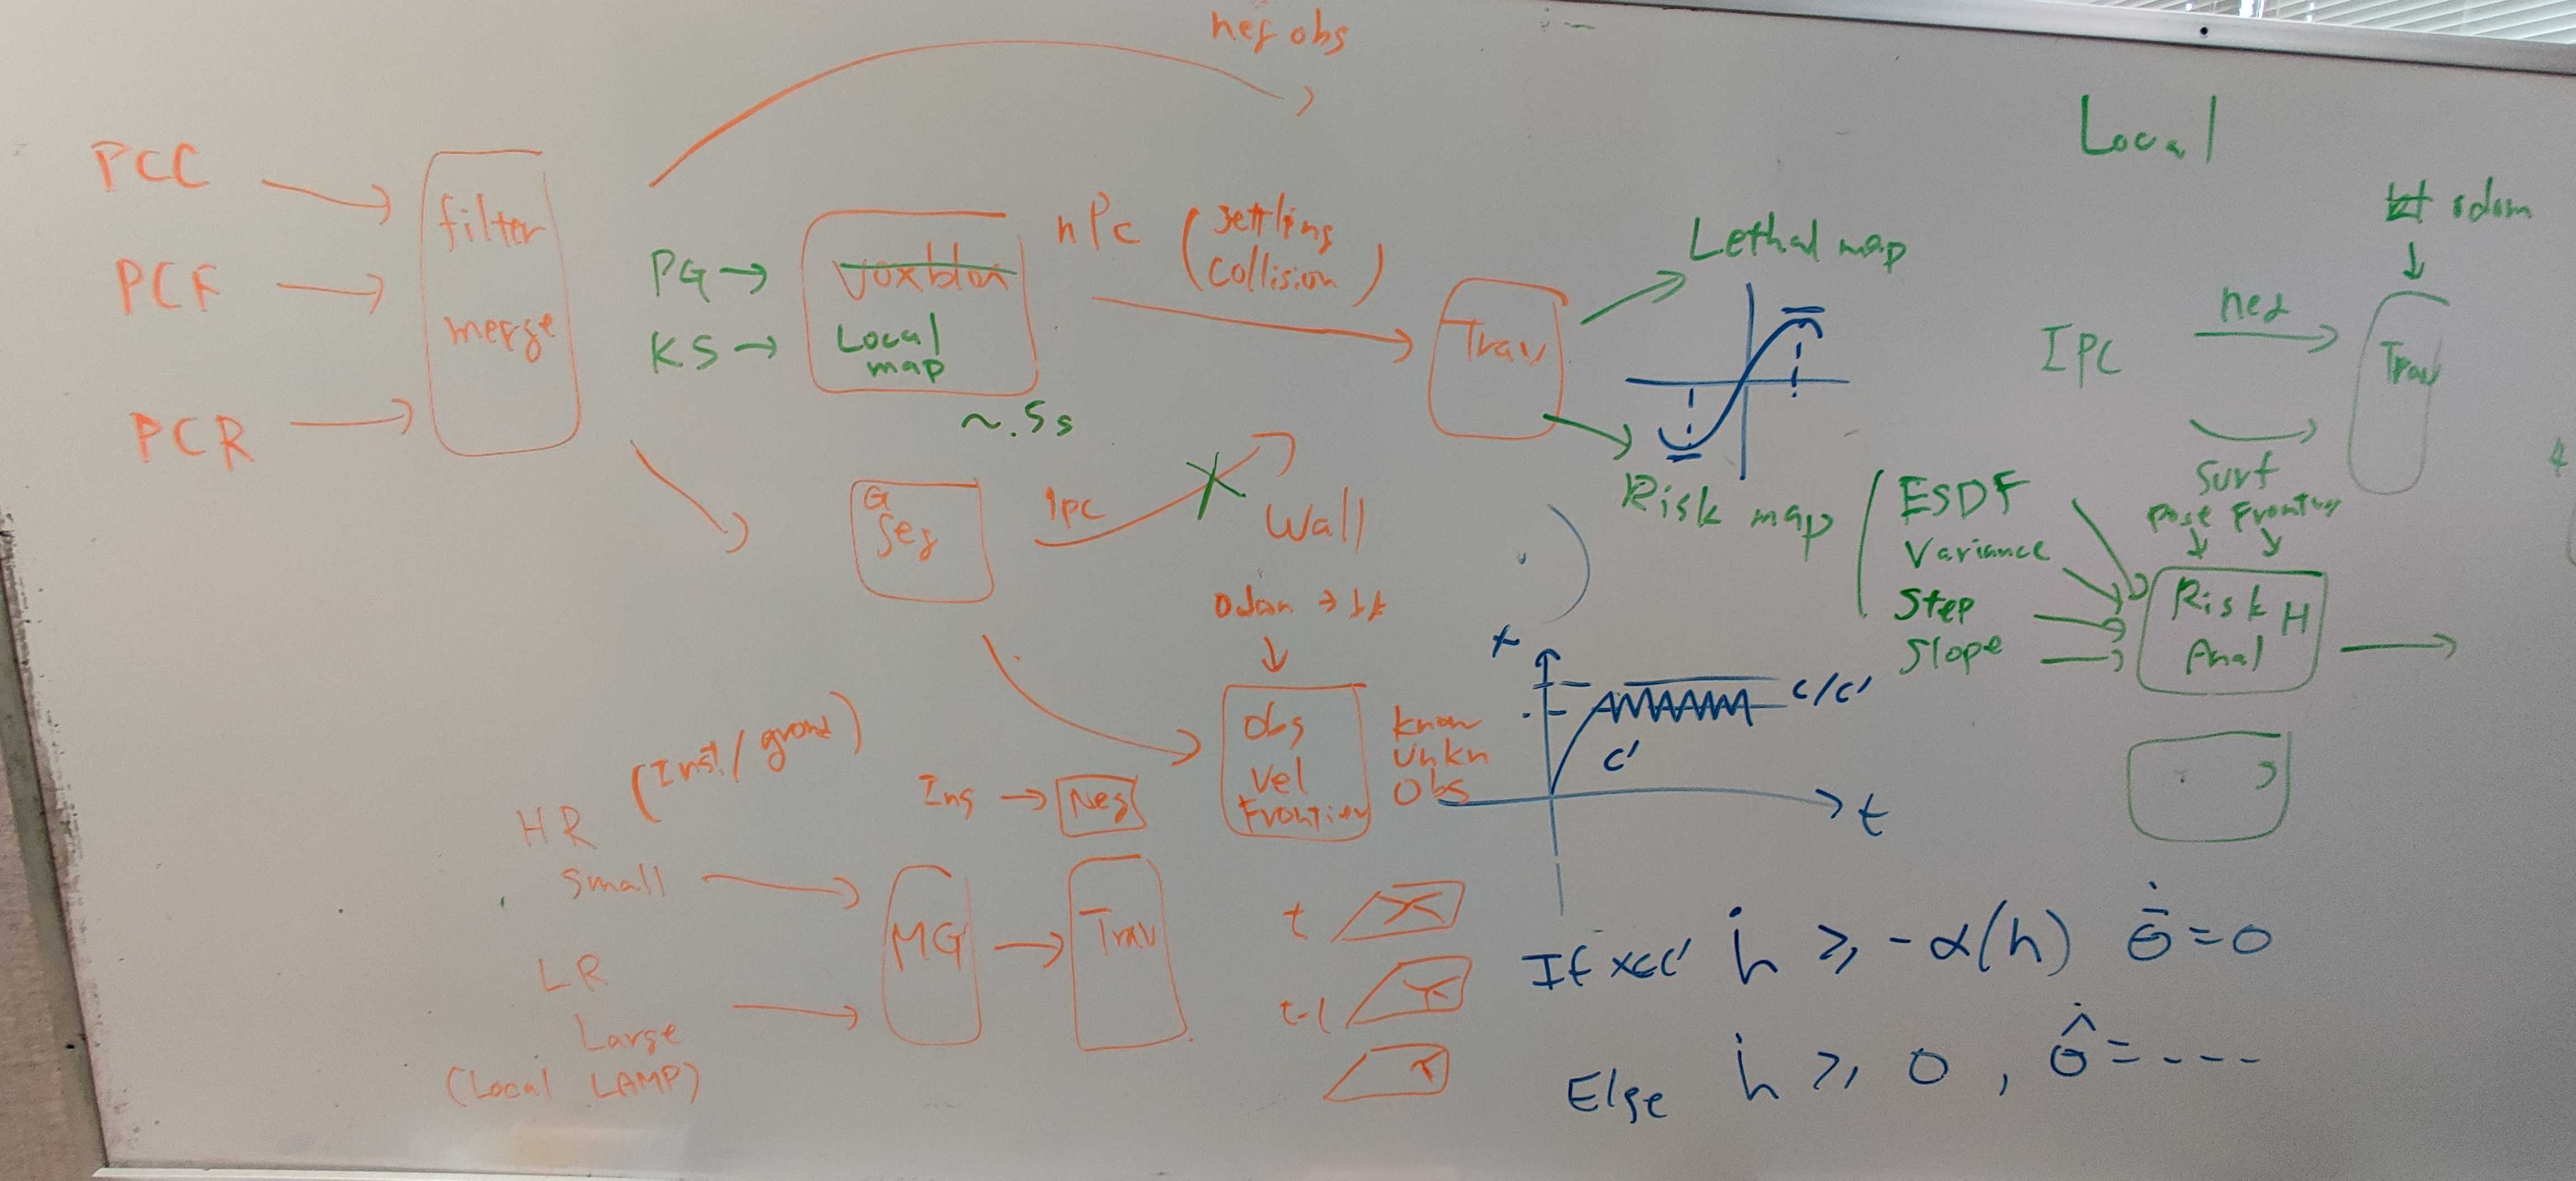
\includegraphics[width=\linewidth]{figs/traversability_notes.jpg}
\end{figure}

% \begin{itemize} % For Mission Autonomy(Behavstmap) -> iours, IRM) probably we just gonna cite Scott and Kyon aero paper. 
%         \item Traversability (settling, collision check, slope check, negative obstacles,..) (David?)
%     \item Local Planning (our traversability/local planner complements BD's internal one. We have long range LiDAR, bigger costmaps and detect negative obstacles. In the local planner, we can encourage forward motion in order to avoid walking into the robot's blind spot and increasing the chance of seeing artifacts with the forward facing sensors)
% \end{itemize}


%%%%%%%%%%%%%%%%%%%%%%%%%%%%%%%%%%%%%%%%%%%%%%%%%%%%%%%%%%%%
\section{Experiments}

%%%%%%%%%%%%%%%%%%%%%%%%%%%%%%%%%%%%%%%%%%%%%%%%%%%%%%%%%%%%
\section{Limitations and Future work}
\begin{itemize}
    \item Relaxing requirement for complete field-of-view (Add image of husky on husky?)
    \item Water
\end{itemize}


%%%%%%%%%%%%%%%%%%%%%%%%%%%%%%%%%%%%%%%%%%%%%%%%%%%%%%%%%%%%
\section{Conclusion}

\begin{figure*}[b]
\centering
\includegraphics[width=.32\textwidth]{figs/arch2.png}\hfill
\includegraphics[width=.32\textwidth]{figs/arch4.png}\hfill
\includegraphics[width=.32\textwidth]{figs/arch3.png}
\caption{default}
\label{fig:figure3}
\end{figure*}

\appendix

\section{BeliefCloud: A Map Representation For Resilient Navigation}
\subsection{Introduction}
\subsection{Literature review}
See \href{https://docs.google.com/spreadsheets/d/11qLnf_ezRuH9mCL2kmDWL4Jrx0DhV9FeSnF24StyZUg/edit#gid=0}{Literature Review}.

See \href{https://docs.google.com/presentation/d/1zdZJyG_-8uM9AR_wMzYOIBy0c8Eg1oV7gbKtXalEBA4/edit#slide=id.g5bf125e9db_6_5}{Traversability slides}

\begin{enumerate}
    \item \cite{InstPcWafr2016} uses instantaneous pointclouds to get robustness to noise in localization but has issues due to occlusions, field-of-view, etc.
    \item \cite{nanomap2018} Nanomap
    \begin{enumerate}
        \item Only use most recent frame in FOV
        \item Does not capture uncertainty in rotation (i.e. important if depth measurements are over a larger distance)
        \item Designed for quadrotor (free space estimation) vs traversabiltiy for ground robots
    \end{enumerate}
    \item Grid based approaches \cite{hornung2013octomap} \cite{agha2017CRM}
    \begin{enumerate}
        \item Need to pick resolution i.e. a trade off between computation and performance.
    \end{enumerate}
    \item \cite{sphericalImage} uses a spherical image to efficiently compute normals
    \item Fitting a plane once we have points with gaussian uncertainty
    \begin{enumerate}
        \item \cite{planeFitUnc2010} shows plane fitting with noise in range measurements of the sensor
        \item \cite{hyperfit2015} shows hyper-plane fitting with general gaussian uncertainty in points
        \item Look at page 5,7 in \href{http://www.desy.de/~blobel/apltalk.pdf}{this link} showing APLCON package. 
        \href{https://github.com/neiser/APLCONpp}{This} is a c++ implementation of it on github with a sample code \href{https://github.com/neiser/APLCONpp}{here}.
    \end{enumerate}
\end{enumerate}

\begin{figure}[t!]
    \centering
    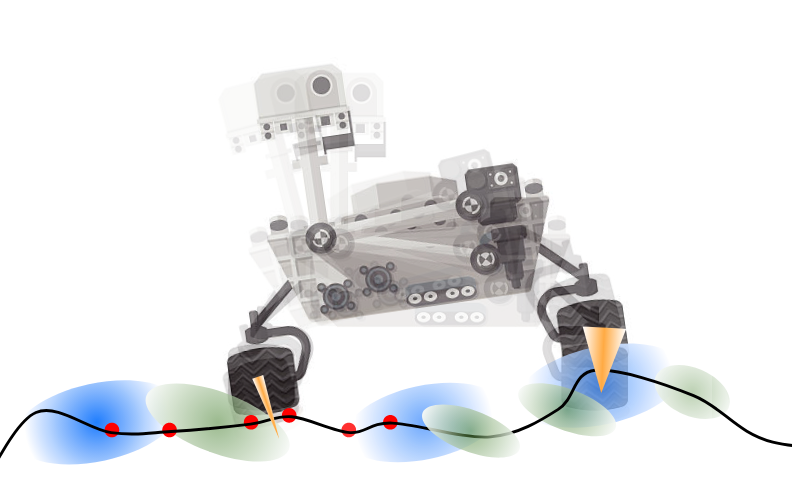
\includegraphics[width=0.95\linewidth]{figs/RoverOnBeliefCloud.png}
    \caption{Stochastic Settling}
    \label{fig:s_settling}
\end{figure}

\begin{figure}[t!]
    \centering
    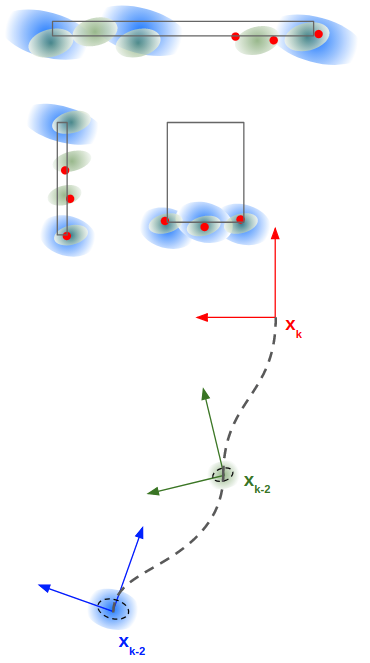
\includegraphics[width=0.65\linewidth]{figs/StochasticMap.png}
    \caption{Stochastic Map}
    \label{fig:s_map}
\end{figure}

\begin{figure}[h!]
    \centering
    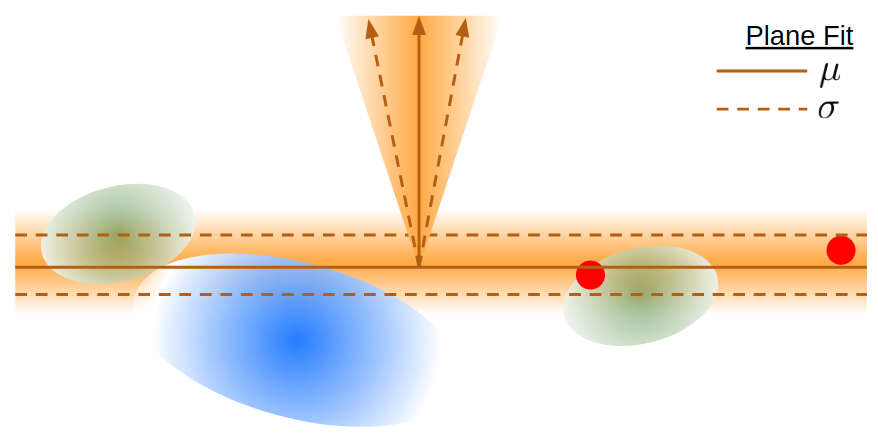
\includegraphics[width=0.95\linewidth]{figs/StochasticPlane.png}
    \caption{Stochastic Plane}
    \label{fig:s_cone}
\end{figure}

\clearpage

\bibliographystyle{unsrt}
\bibliography{ref}

\clearpage

\section{Discussion}
\subsection{Motivation}
Inst Point Clouds --> don't keep history (bad), but no noise (good)
Voxblox --> don't consider error in state estimation, everything in world frame

Many times the planner only needs to plan in the local frame, not in the world frame. 

\subsection{Key Ideas}
\begin{itemize}
    \item Larger tolerance for things that are far away
    \item Plan in current body frame and inflate the covariance of previous estimate (degenerate to instant. pointclouds when using bad localization source)
    \item landing on form (stochastic traversability)
    \item Account for uncertainty in pitch
    
    \item \textbf{How estimation error is modelled?}
    \begin{itemize}
		\item Take the covariances from the estimation algorithm? 
		\item based on $v, a, \omega$
	\end{itemize}

    \item \textbf{How sensor noise is modelled?}
    \begin{itemize}
		\item Find specific model for Velodyne, depth sensor,... \jesus{I don't like too much this idea, we will end up with an algorithm that will require experiments to find the sensor model for every different sensor. Would it be possible to find this in an online fashion? Or just at the start of each run, with the robot still, compute the variance in each direction (but this may not work to compute the bias wrt the ground truth?)}
		\rohan{The idea is that you would only do this once per sensor. E.g. point the velodyne to a flat wall at a known distance and fit a plane and characterize the sensor noise.}
	\end{itemize}

    \item \textbf{How covariances are propagated backwards?}
    \begin{itemize}
		\item The previous frame, expressed in the current frame, has translation ~Distribution(mean, variance) and rotation ~Distribution(mean, variance)
		\item Nanomap propagates only translation, but not rotation (and therefore the propagation is linear). Propagating both is not linear--> we should find a way to efficiently approximate this. 
		\rohan{see \cite{barfoot2014associating} \cite{se3unc} but can directly use \href{http://wiki.ros.org/pose_cov_ops}{pos\_cov\_ops ros package}}.
	\end{itemize}

    \item \textbf{Representation}
    \begin{itemize}
		\item Brute Force 1: for every point of every point cloud $n=0,...,n=N-1$, keep mean (3 values), and covariance (other 3 values).
		
		\item \textbf{Selective choice} of the 
		
		\begin{itemize}
		    \item $N$ point clouds that will be used to compute the fused map: If the robot is still, take few point clouds from that moment, but many point clouds when the robot was moving.  
		    \item Area of the point cloud that will be used: If two point clouds overlap, take points in that area corresponding to the point cloud closer to the current frame (i.e. point cloud with smaller $n$).
		\end{itemize}
		
		Once the selective choice has been made, we end up with a single point cloud that contains points from every point cloud. As we have now the uncertainty in position and orientation of the frame of the lidar where that point was captured, we can compute the uncertainty in position of a specific point wrt to the frame $n=0$
		
		\begin{figure}
		    \centering
		    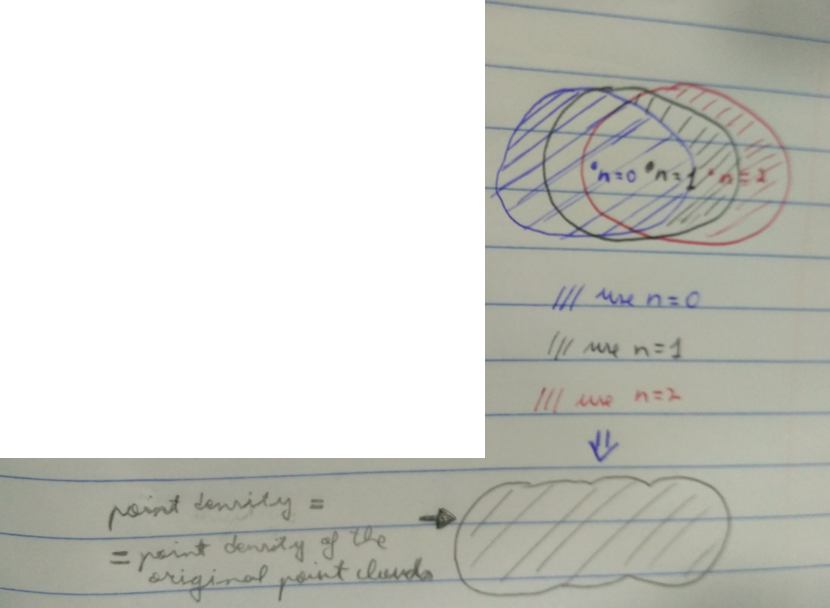
\includegraphics[width=\columnwidth]{./figs/traversability3.PNG}
		    \caption{Selective Selection}
		    \label{fig:my_label}
		\end{figure}
		
		\item Should we compute everything from scratch in every iteration? (i.e. should we fuse the $N$ selected point clouds in every iteration) or is there a way to reuse past computation?
	\end{itemize}

    \item \textbf{Traversability computation}
    
        \begin{itemize}
		\item Take into account different yaws of the vehicle for the same point? (and not just the same orientation for the same point, as we are doing right now)
		\item Stochastic normal estimation
		\begin{itemize}
		    \item Brute force 1:  for every point (random variable), sample a point--> obtain a surface, and compute the normal  from this surface. Obtain a traversability value (# of points inside the box?) from this surface. Note that the points inside that box are also random variables. We could do something like traversability= intersection of the pdf of the box with the pdfs of the points / total volume of the box
		    Do this several times, and the traversability mean and deviation are obtained from this sampling.
		    
		    Traversability should be a continuous value, not a boolean one (right now it's yes or no). 
		    \item The stochastic normal estimation should be a distribution over a 3d unit sphere (https://en.wikipedia.org/wiki/Kent_distribution)
		\end{itemize}
		
		\begin{figure}
		    \centering
		    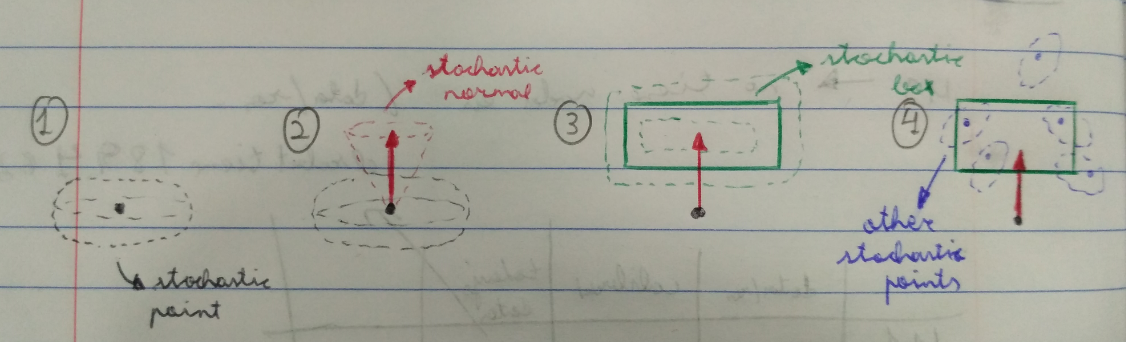
\includegraphics[width=\textwidth]{./figs/stochastic_trav.PNG}
		    \caption{Caption}
		    \label{fig:my_label}
		\end{figure}
		
	\end{itemize}

    \item \textbf{Output} The output should be an stochastic traversability value ~Distribution(mean, variance). Could planners benefit from this random variable (similar to CRM from Ali) or should we just keep the mean? 
    
\end{itemize}



\bibliographystyle{unsrt}
\bibliography{ref}

\end{document}